\subsection*{Ejercicio 4. El Escalograma (CWT)} %
El electrocardiograma que viene en la librería \texttt{scipy.misc} es el usado por que es un ejemplifica bien un tupo de señal no estacionaria

\vspace{0.5cm}
\noindent \textbf{1 y 2. Señal original en el dominio del tiempo} %

Calculo la CWT de la señal original del electrocardiograma usando una wavelet madre de Morlet

\begin{figure}[H]
    \centering
    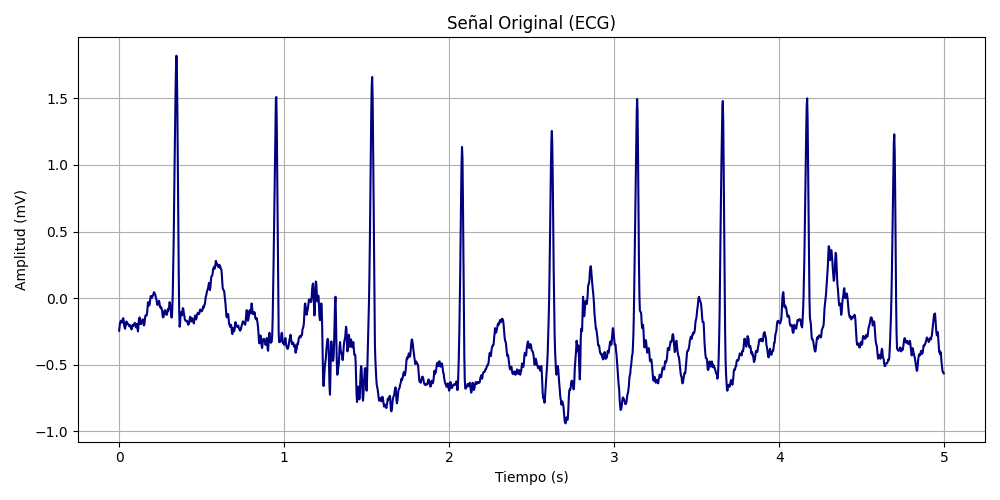
\includegraphics[width=0.8\textwidth]{figuras/ej4_senal_original.png} 
    \caption{Señal real de electrocardiograma no estacionaria.}
\end{figure}

\noindent \textbf{3. Escalograma Resultante} %

\begin{figure}[H]
    \centering
    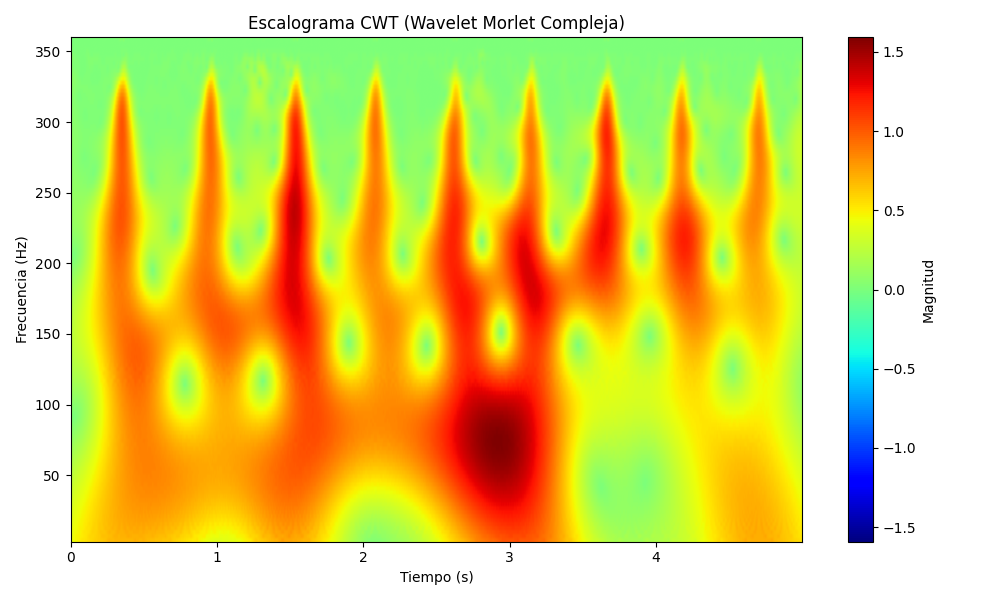
\includegraphics[width=0.8\textwidth]{figuras/ej4_escalograma.png} 
    \caption{Escalograma de la señal ECG utilizando wavelet de Morlet compleja Y es la frecuencia en Hz y el color indica la magnitud de los coeficientes.}
\end{figure}

\vspace{0.5cm}
\noindent \textbf{4. Identificación de eventos transitorios} %

Notemos que hay eventos transitorios que Fourier no mostraria
\begin{itemize}
    \item \textbf{Latido del corazón:} Aparece de forma periódica alrrededoir de 0.8 segundos que se ve en las franjas verticales muy intensas que van en frecuencias entre 10 Hz y 40 Hz notesé que el eje temporal se ven los picos del ECG 
    \item \textbf{Ondas P y T:} Antes y después de cada uno de estos complejos QRS se ven ven manchas aisladas de energía en frecuencias muy bajas que mustran cuando los ventrículos se despolarizan y repolarizan.
\end{itemize}

Si se tratara esto con un espectro de Fourier tradicional tendriamos que hay un montón de actividad entre 1 Hz y 40 Hz, pero no sabemos cuando latió el corazón. Pero, por otro lado el escalograma si nos muestra casi bastante precisamente cuándo ocurre cada pico y con qué frecuencias lo hace
